\subsubsection{Reproducibility} \label{odp_reproducibility}
% Subsection structure:
% Problem: what is the generalized problem?
% 	Motivation: why is this problem scientifically important and/or interesting?
% Solution: conceptual description of solution, including formal definition of GODP and SHACL shapes.
% 	Illustration: images of GODP structure.
% 	(Statistical)Analysis: how does the solution solve the problem?
% 	Evaluation: are the results significant? What is the impact?
\paragraph{Detecting reproducibility}
We use reproducibility to evaluate the reliability of decision-relevant information. The reproducibility pattern can detect when information cannot be traced back to an evidence source. When evidence cannot be traced back to an evidence source, the pattern detects the information as premature. 

\begin{center}
\large\color{document}{The reproducibility pattern validates the information reliability by detecting when information cannot be traced back to an evidence source.}
\end{center}

\paragraph{Ontology}
Information is reproducible when it can be traced back to evidence or an information source, for example, a contextual circumstance or the value of a stakeholder. This pattern relates information to an evidence source using an object property. An information class can be based on another information class as well, as long as the chain of information is evidence-based. We use the completeness pattern to ensure the required data properties are available. Figure \ref{fig:reproducibility_chain} presents a chain that connects information to evidence. The $based\_on\_in{\f}ormation$ object property is transitive. When we base information $a$ on information $b$, and information $b$ on information $c$, then information $a$ is also based on information $c$. We need the transitive characteristic to query the evidence sources of information for the decision presentation pattern.

\begin{figure}[H]
\centering
  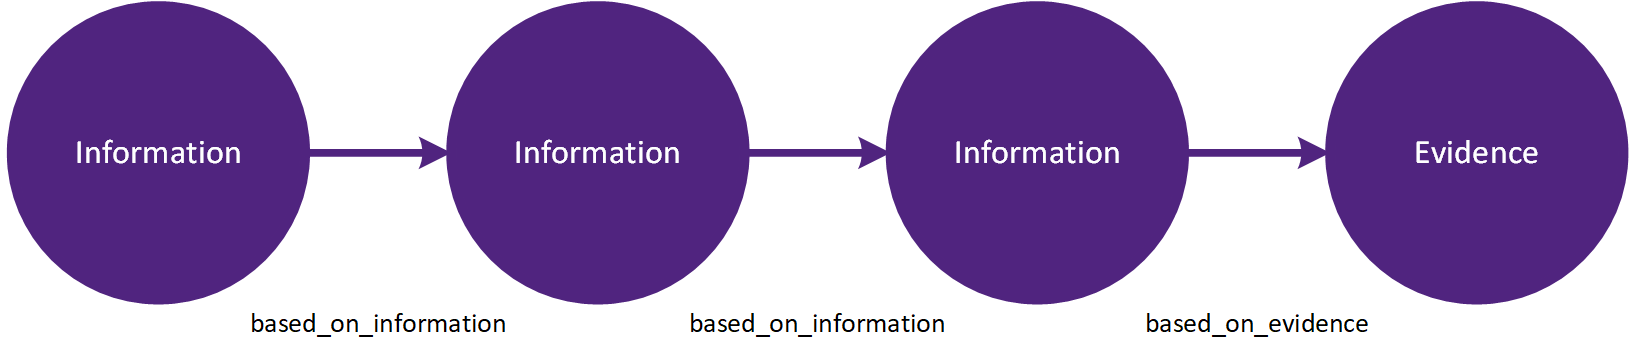
\includegraphics[width=13cm]{../../Images/Reproducibility_Chain.png}
  \caption{An example of an evidence-based chain of information. The reproducibility pattern should detect if the information in the chain is not evidence-based.}
  \label{fig:reproducibility_chain}
\end{figure} 

We extend the evidence-based management pattern in two ways:
\begin{enumerate}
\item Contextual circumstances and evaluated external evidence naturally refer to their actual evidence source, for example, a scientific article or an observation. Stakeholder evidence requires a specific stakeholder as a source of evidence. We extend the evidence-based management pattern with one class ($Stakeholder$) and the related object property ($shared\_by$). 
\item Individuals (classified as $In{\f}ormation$) hosting data properties should be evidence-based or information-based. The object property $based\_on\_evidence$ relates a class to the evidence class. The object property $based\_on\_in{\f}ormation$ relates a class to an information class. 
\end{enumerate} 

Figure \ref{fig:reproducibility} presents the resulting ontology. We have marked the extensions of the evidence-based management pattern in \textcolor{DarkBlue}{blue}.

\begin{figure}[H]
\centering
  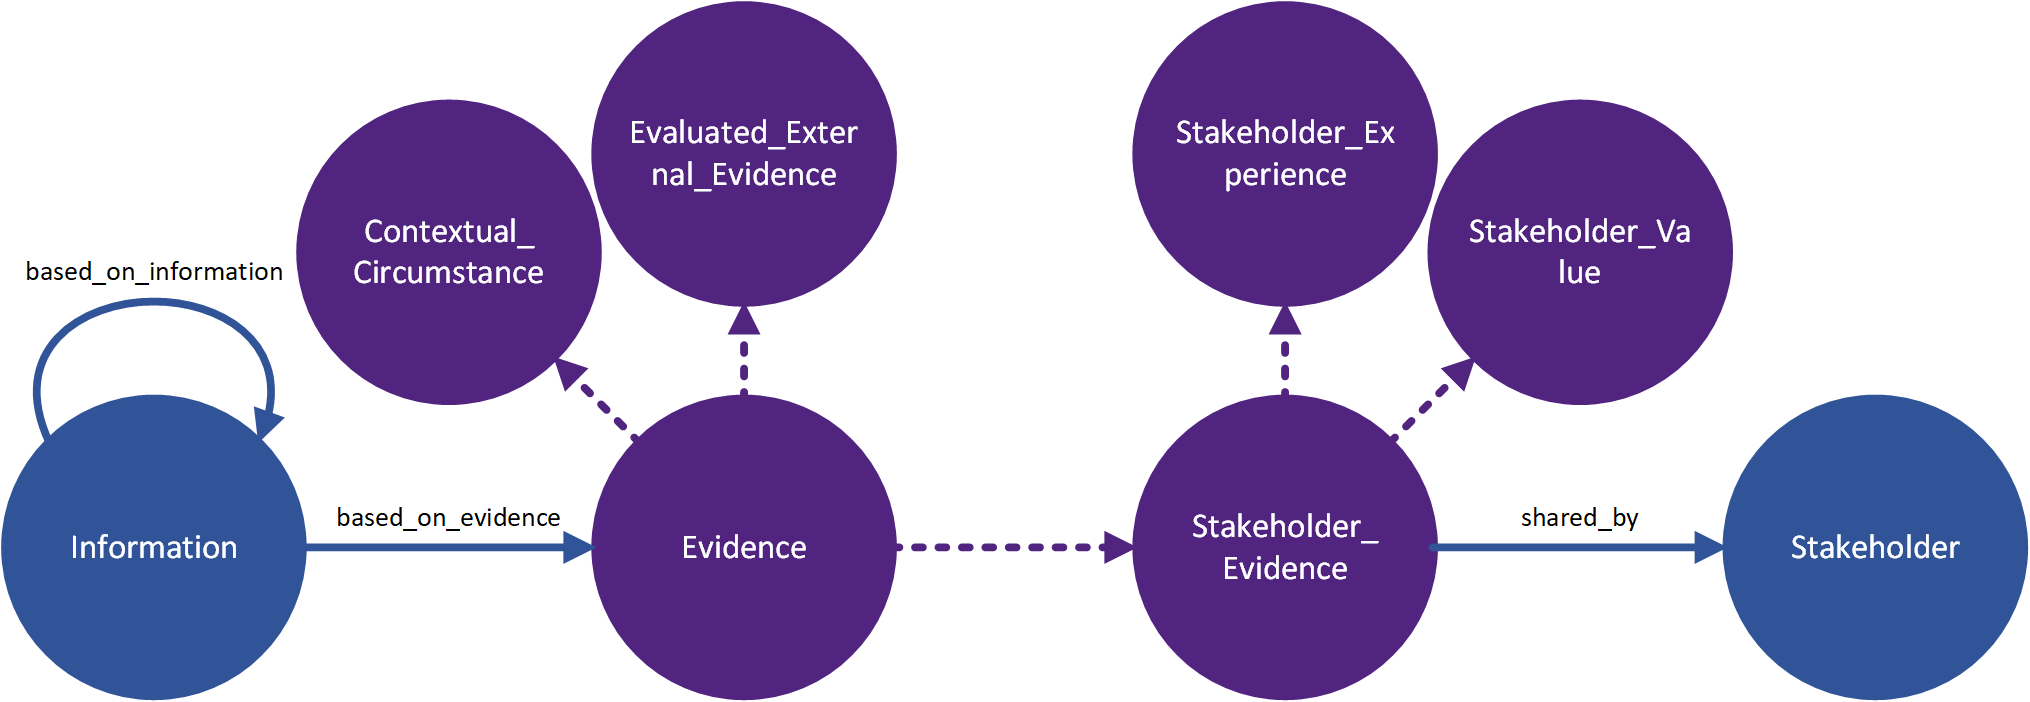
\includegraphics[width=14cm]{../../Images/04_Contribution/04_Reproducibility_Ontology.png}
  \caption{The reproducibility ontology. We have marked the extensions of the evidence-based management pattern in \textcolor{DarkBlue}{blue}. Code sample \ref{GODP_REP_EXT} presents the GDOL code that we use to instantiate this pattern.}
  \label{fig:reproducibility}
\end{figure}

\paragraph{Inferencing}
We use the domain and range of the $based\_on\_information$, $based\_on\_evidence$, and $shared\_by$ object properties to allow the reasoner to classify individuals that are using these object properties. Table \ref{table:rep_inference} presents the classification the reasoner infers from the domain and range configuration.

\begin{table}[H]
\centering
\caption{We use the domain and range of the $based\_on\_in{\f}ormation$, $based\_on\_evidence$, and $shared\_by$ object properties to allow the reasoner to classify individuals that are using these object properties.}
\begin{tabular}{| p{4cm} | p{6cm} |  p{4cm} |   }
\hline
\rowcolor{document}
\color{documentText}Domain & \color{documentText}Object property & \color{documentText}Range \\
\hline
$In{\f}ormation$ & $based\_on\_in{\f}ormation$ & $In{\f}ormation$ \\
\hdashline
$In{\f}ormation$ & $based\_on\_evidence$ & $Evidence$ \\
\hdashline
$Stakeholder\_Evidence$ & $shared\_by$ & $Stakeholder$ \\
\hline
\end{tabular}
\label{table:rep_inference}
\end{table}

\paragraph{Inconsistency} \label{rep_incons}
We guard the consistency of the ontology using $DisjointClasses$. The reasoner cannot classify an individual as $Information$ and $Evidence$ at the same time. If we allow the reasoner to do this, it might create a circular dependency in the reproducibility chain figure \ref{fig:reproducibility_chain} presents. $In{\f}ormation$ typically represents a statement that we can trace back to at least one $Evidence$ source. Code sample \ref{GODP_REP_EXT} presents the implementation of the $DisjointClasses$.

\paragraph{Generic ontology design pattern}
Figure \ref{fig:reproducibility} presents an ontology that extends the evidence-based management ontology and enables the detection of unreproducible information. Code sample \ref{GODP_REP_EXT} presents the GDOL code that extends the evidence-based management ontology. 

\begin{lstlisting}[float,language=GDOL,caption={The GDOL code for relating information to evidence and stakeholder evidence to a stakeholder. We introduce two new classes ($Stakeholder$ and $Information$) and three new object properties ($shared\_by$, $based\_on\_evidence$, and $based\_on\_in{\f}ormation$. Additionally, we define that $Information$ and $Evidence$ are disjoint. Figure \ref{fig:reproducibility} visualises the result of executing the code.},label={GODP_REP_EXT}][H]
ontology Reproducibility_Basic = EBM then 
 Class: Stakeholder 
 Class: Information 
 ObjectProperty shared_by Domain: Stakeholder_Evidence Range: Stakeholder 
 ObjectProperty based_on_evidence Domain: Information Range: Evidence
 ObjectProperty based_on_information Domain: Information Range: Information Characteristics: Transitive
 DisjointClasses: Information, Evidence
\end{lstlisting}

The classes that store decision-relevant information are required to be a subclass of $In{\f}ormation$. Code sample \ref{GODP_REP_EV} presents the GDOL code that relates information to evidence. The inferencing using the domain and range of the $based\_on\_in{\f}ormation$, $based\_on\_evidence$, and $shared\_by$ object properties contributes to this classification as well.

\begin{lstlisting}[float,language=GDOL,caption={The GDOL code that classifies individuals as a sub-class of $Information$. We use $dri$ (decision relevant information) and $i$ (information) as parameters.},label={GODP_REP_EV}][H]
pattern Reproducibility_Context [Class: dri; Class: i] = 
 Class: [dri] SubClassOf: [i]
\end{lstlisting}

\paragraph{Constraints}
Code sample \ref{SHACL_REP} presents the SHACL shape that detects unreproducible information. Each individual that is classified as $In{\f}ormation$ is required to host the object property $based\_on\_in{\f}ormation$ or $based\_on\_evidence$. Individuals that are classified as $In{\f}ormation$ can be traced back to an evidence or information source by hosting one of these two object properties. If the individual does not host one of the object properties, its information cannot be traced back to an evidence source, and the pattern detects the information as premature. The SHACL shape monitors the existence of the object properties using the cardinality constraint $minCount$. 

\begin{lstlisting}[float,language=SHACL,caption={The SHACL code that detects if $Information$ is not $based\_on\_evidence$ or $based\_on\_in{\f}ormation$. The SHACL shape monitors the existence of these object properties using the cardinality constraint $minCount$. },label={SHACL_REP}][H]
Used_InformationShape a sh:NodeShape;
	sh:targetClass Information; 
	sh:property [
		sh:or (
			[sh:path based_on_information; sh:minCount 1;]
			[sh:path based_on_evidence; sh:minCount 1;]
		)
		sh:severity sh:Violation; 
		sh:message "Reproducibility: enter an information or evidence source for this information."; ];
\end{lstlisting}

Code sample \ref{SHACL_REP_SH} presents the SHACL shape that detects when the pattern cannot trace back $Stakeholder\_Experience$ or a $Stakeholder\_Value$ to a $Stakeholder$. We use the $shared\_by$ combined with the cardinality constraints $sh:minCount$ object property to achieve this. The constraints generate a violation if an individual that is classified as $Stakeholder\_Evidence$ is not $shared\_by$ a stakeholder.

\begin{lstlisting}[float,language=SHACL,caption={The SHACL code that detects when a stakeholder does not share $Stakeholder\_Evidence$. We use the cardinality constraint $sh:minCount$ for this detection: each individual classified as $Stakeholder\_Evidence$ should have at least one path $shared\_by$. The range of $shared\_by$ is $Stakeholder$.},label={SHACL_REP_SH}][H]
StakeholderShape a sh:NodeShape;
	sh:targetClass Stakeholder_Evidence; 
	sh:property [
		sh:path shared_by;
		sh:severity sh:Violation; 
		sh:minCount 1; 
		sh:message "Reproducibility: enter a stakeholder that serves as the source of this stakeholder evidence."; ];
\end{lstlisting}